% This is samplepaper.tex, a sample chapter demonstrating the
% LLNCS macro package for Springer Computer Science proceedings;
% Version 2.21 of 2022/01/12
%
\documentclass[runningheads]{llncs}
%
\usepackage[T1]{fontenc}
% T1 fonts will be used to generate the final print and online PDFs,
% so please use T1 fonts in your manuscript whenever possible.
% Other font encondings may result in incorrect characters.
%
\usepackage{graphicx}
\usepackage{hyperref} 
\usepackage{amsmath}
\usepackage{mathabx}
\usepackage[printonlyused,withpage]{acronym}

% Used for displaying a sample figure. If possible, figure files should
% be included in EPS format.
%
% If you use the hyperref package, please uncomment the following two lines
% to display URLs in blue roman font according to Springer's eBook style:
%\usepackage{color}
%\renewcommand\UrlFont{\color{blue}\rmfamily}
%\urlstyle{rm}
%
\begin{document}
%
\title{MiniSat Report}
%
%\titlerunning{Abbreviated paper title}
% If the paper title is too long for the running head, you can set
% an abbreviated paper title here
%
\author{Șova Dumitru Ștefan Andrei \href{dumitru.sova01@e-uvt.ro}{dumitru.sova01@e-uvt.ro} \\
   \and Andries Rafael Gabriel \href{mailto:rafael.andries00@e-uvt.ro}{rafael.andries00@e-uvt.ro} \\
   \and Stoentel Alexandru-Eduard \href{mailto:alexandru.stoentel01@e-uvt.ro}{alexandru.stoentel01@e-uvt.ro} \\
   \and Nenescu Eugeniu \href{mailto:eugeniu.nenescu00@e-uvt.ro}{eugeniu.nenescu00@e-uvt.ro} }
%
\authorrunning{F. Author et al.}
% First names are abbreviated in the running head.
% If there are more than two authors, 'et al.' is used.
%
\institute{West University of Timișoara, Bulevardul Vasile Pârvan 4, Timișoara 300223}
%
\maketitle              % typeset the header of the contribution
%
\begin{abstract}

Since time immemorial, logic has helped us make sense of the world that surrounds us, from our ancestors' philosophical inquiries to its use in modern mathematics and informatics. Logic bridges the gap between formal and informal knowledge, proving essential in fields as diverse as databases, programming languages (\ac{e.g.}, Prolog), and propositional logic. This paper focuses on a compelling area within informatics: the \ac{SAT}, a foundational challenge in computational complexity. \ac{SAT} asks whether a set of variable assignments can satisfy a Boolean formula and stands as the first problem proven to be \ac{NP-complete}. Our main focus will be on MiniSat, an \ac{SAT} solver designed to address this challenge efficiently. Finally, such solvers enabled tackling practical problems with millions of variables, benefiting research and industry.

This report includes benchmarks from recent \ac{SAT} competitions, alongside minor modifications to MiniSat’s original code, to compare results and evaluate its performance across different problem instances. With time results and outputs available on GitHub, this analysis highlights MiniSat’s capabilities and underscores the broader impact of \ac{SAT} solvers in advancing computational problem-solving. GitHub link for the project: \url{https://github.com/AndiSova/VF-Software-Engineering-2024-Project}

\keywords{MiniSat  \and \ac{SAT} \and logic.}
\end{abstract}

\newpage
%
%
%
\section{Introduction}

\ac{SAT} is a cornerstone in computational theory and practical applications, namely \ac{EDA}, artificial intelligence, and combinatorial optimization (see \cite{sat-solver}). Since 2003, MiniSat has continued to be a small, efficient, and readable \ac{SAT} solver, representing a perfect tool to introduce students and professionals alike to the nuances of \ac{SAT} solving (see \cite{minisat}).

While MiniSat is often praised for its straightforward design, working with it as a beginner can present various challenges. For instance, setting up MiniSat, understanding its underlying algorithms, such as \ac{DPLL} and \ac{CDCL}, and configuring it for experimental benchmarks requires both theoretical and practical knowledge. In addition, interpreting MiniSat’s internal workings can be challenging, as it demands familiarity with conflict-driven clause learning, unit propagation, and constraint management, all of which are fundamental to modern \ac{SAT} solvers’ efficiency.

In this report, we will explore these challenges from the perspective of newly introduced users. Our study includes the steps for installing MiniSat, configuring it to run benchmarks from the \ac{SAT} competition, and analyzing the results. We’ll also delve into the algorithms that power MiniSat, examining ways they could be enhanced. Throughout, we apply principles from software engineering, using \ac{UML} diagrams and detailed code documentation to bridge the gap between theoretical concepts and practical implementation. This report aims to provide a comprehensive overview for those new to SAT solvers, emphasizing the complexities and rewards of exploring this powerful problem-solving tool.
 

\subsection{Motivation}

Our motivation for studying MiniSat stems from its influential role in advancing \ac{SAT} solver technology and its accessibility as a learning tool. MiniSat has not only set a standard for efficiency in solving \ac{SAT} problems but also provides a straightforward and readable code that allows us to delve into its algorithms and structure. It represents a perfect starting line for our introduction into the world of \ac{SAT} solvers and their particularities, allowing us to understand key \ac{SAT}-solving techniques like \ac{DPLL} and \ac{CDCL} and explore potential improvements in these areas. By examining MiniSat’s contributions and considering modifications, we aim to gain a deeper appreciation of SAT solvers' impact on fields like AI, optimization, and verification.

\newpage

\section{SAT problem and solutions}
\subsection{Problem description}

The \ac{SAT} problem in propositional logic asks to determine in a given formula that combines atomic propositions using the Boolean operators "and" ($\land$), "or" ($\lor$), and "not" ($\neg$), whether there are truth values for the atoms in the formula such that the formula evaluates to true. Formally, \ac{SAT} is the challenge of determining if a logical formula, typically represented in \ac{CNF}, has at least one solution.

While possible to be resolved by hand, after a certain number of atoms, the solution for such formulas becomes increasingly harder to be determined by ourselves alone, resulting in the need for such solvers to exist. This challenge has fueled the development of specialized \ac{SAT} solvers, which apply advanced algorithms to efficiently handle these vast and intricate formulas.

With \ac{SAT} solvers like MiniSat, which are designed specifically to tackle these computational hurdles, we reached a level where it is feasible to solve \ac{SAT} problems within a reasonable timeframe, even as formula complexity scales up. Because of its ease of modifiability, we will look in this paper at ways that we could improve the current code and compare our results with the original.

\subsection{MiniSat installation and first challenges}

To begin using MiniSat on our Windows machines, we opted for the \ac{WSL} approach, which allows us to run a Linux environment natively on Windows without the need for virtual machines or terminals such as Cygwin. Below are the steps followed for the installation process:

Here are the steps for installing \ac{WSL} and Ubuntu: To enable \ac{WSL}, we ran the command \begin{verbatim}wsl --install\end{verbatim} in PowerShell, running it as an Administrator. This command installs the required features and the default Linux distribution (Ubuntu) for \ac{WSL}. However, in some cases, users may encounter issues where the installation hangs or doesn't complete. To resolve this, it's necessary to ensure that Windows is fully updated and that the proper components for \ac{WSL} 2 are manually enabled. This can be done using PowerShell commands like \begin{verbatim}dism.exe\end{verbatim} to enable \ac{WSL} and Virtual Machine Platform features. After completing the steps, the \begin{verbatim}wsl --set-default-version 2 \end{verbatim}  command was run to ensure \ac{WSL} 2 was set as the default version.

Installing MiniSat on Ubuntu: Once Ubuntu was installed from the Microsoft Store(not necessary, Ubuntu can also be installed from its home site as well, Microsoft Store was used for convenience) and set up with a username and password, the installation of MiniSat was straightforward. First, we updated the package list using the command: \begin{verbatim}sudo apt update\end{verbatim} Next, we installed the MiniSat solver by running: \begin{verbatim}sudo apt install minisat\end{verbatim}

With MiniSat successfully installed, we can run the solver and evaluate its performance. To ensure that MiniSat is working properly, we can first test its basic functionality by running a sample input. To do this, we simply need to open the Ubuntu terminal and type the following command: \begin{verbatim}minisat\end{verbatim} This should display MiniSat’s usage instructions, confirming that the installation was indeed successful.

\begin{figure}
\centering
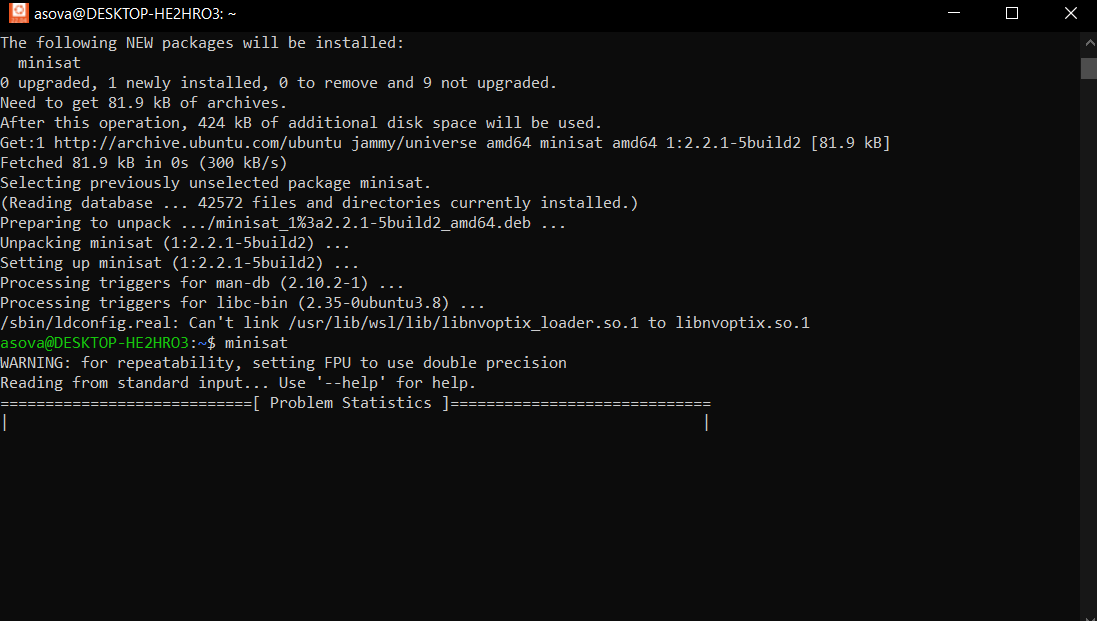
\includegraphics[width=12cm, height=5.7cm]{fig.1.png}
\caption{Successfully installation of MiniSat.} 
\label{fig1}
\end{figure}

Next, to run a benchmark, we use test instances from recent SAT competitions. These competitions provide challenging SAT instances that can be used to evaluate the efficiency and performance of various solvers, including MiniSat.

To run a benchmark, we can follow these steps:

Firstly, we need to download the benchmark files, they are typically available from SAT competition websites, such as \url{https://satcompetition.github.io/2024/} or \url{https://benchmark-database.de/?track=main_2024}.

Having downloaded a benchmark file (usually in .cnf format), we can use the following command to run MiniSat on it: \begin{verbatim}
minisat <benchmark_file>.cnf result.txt
\end{verbatim}

\begin{figure}
\centering
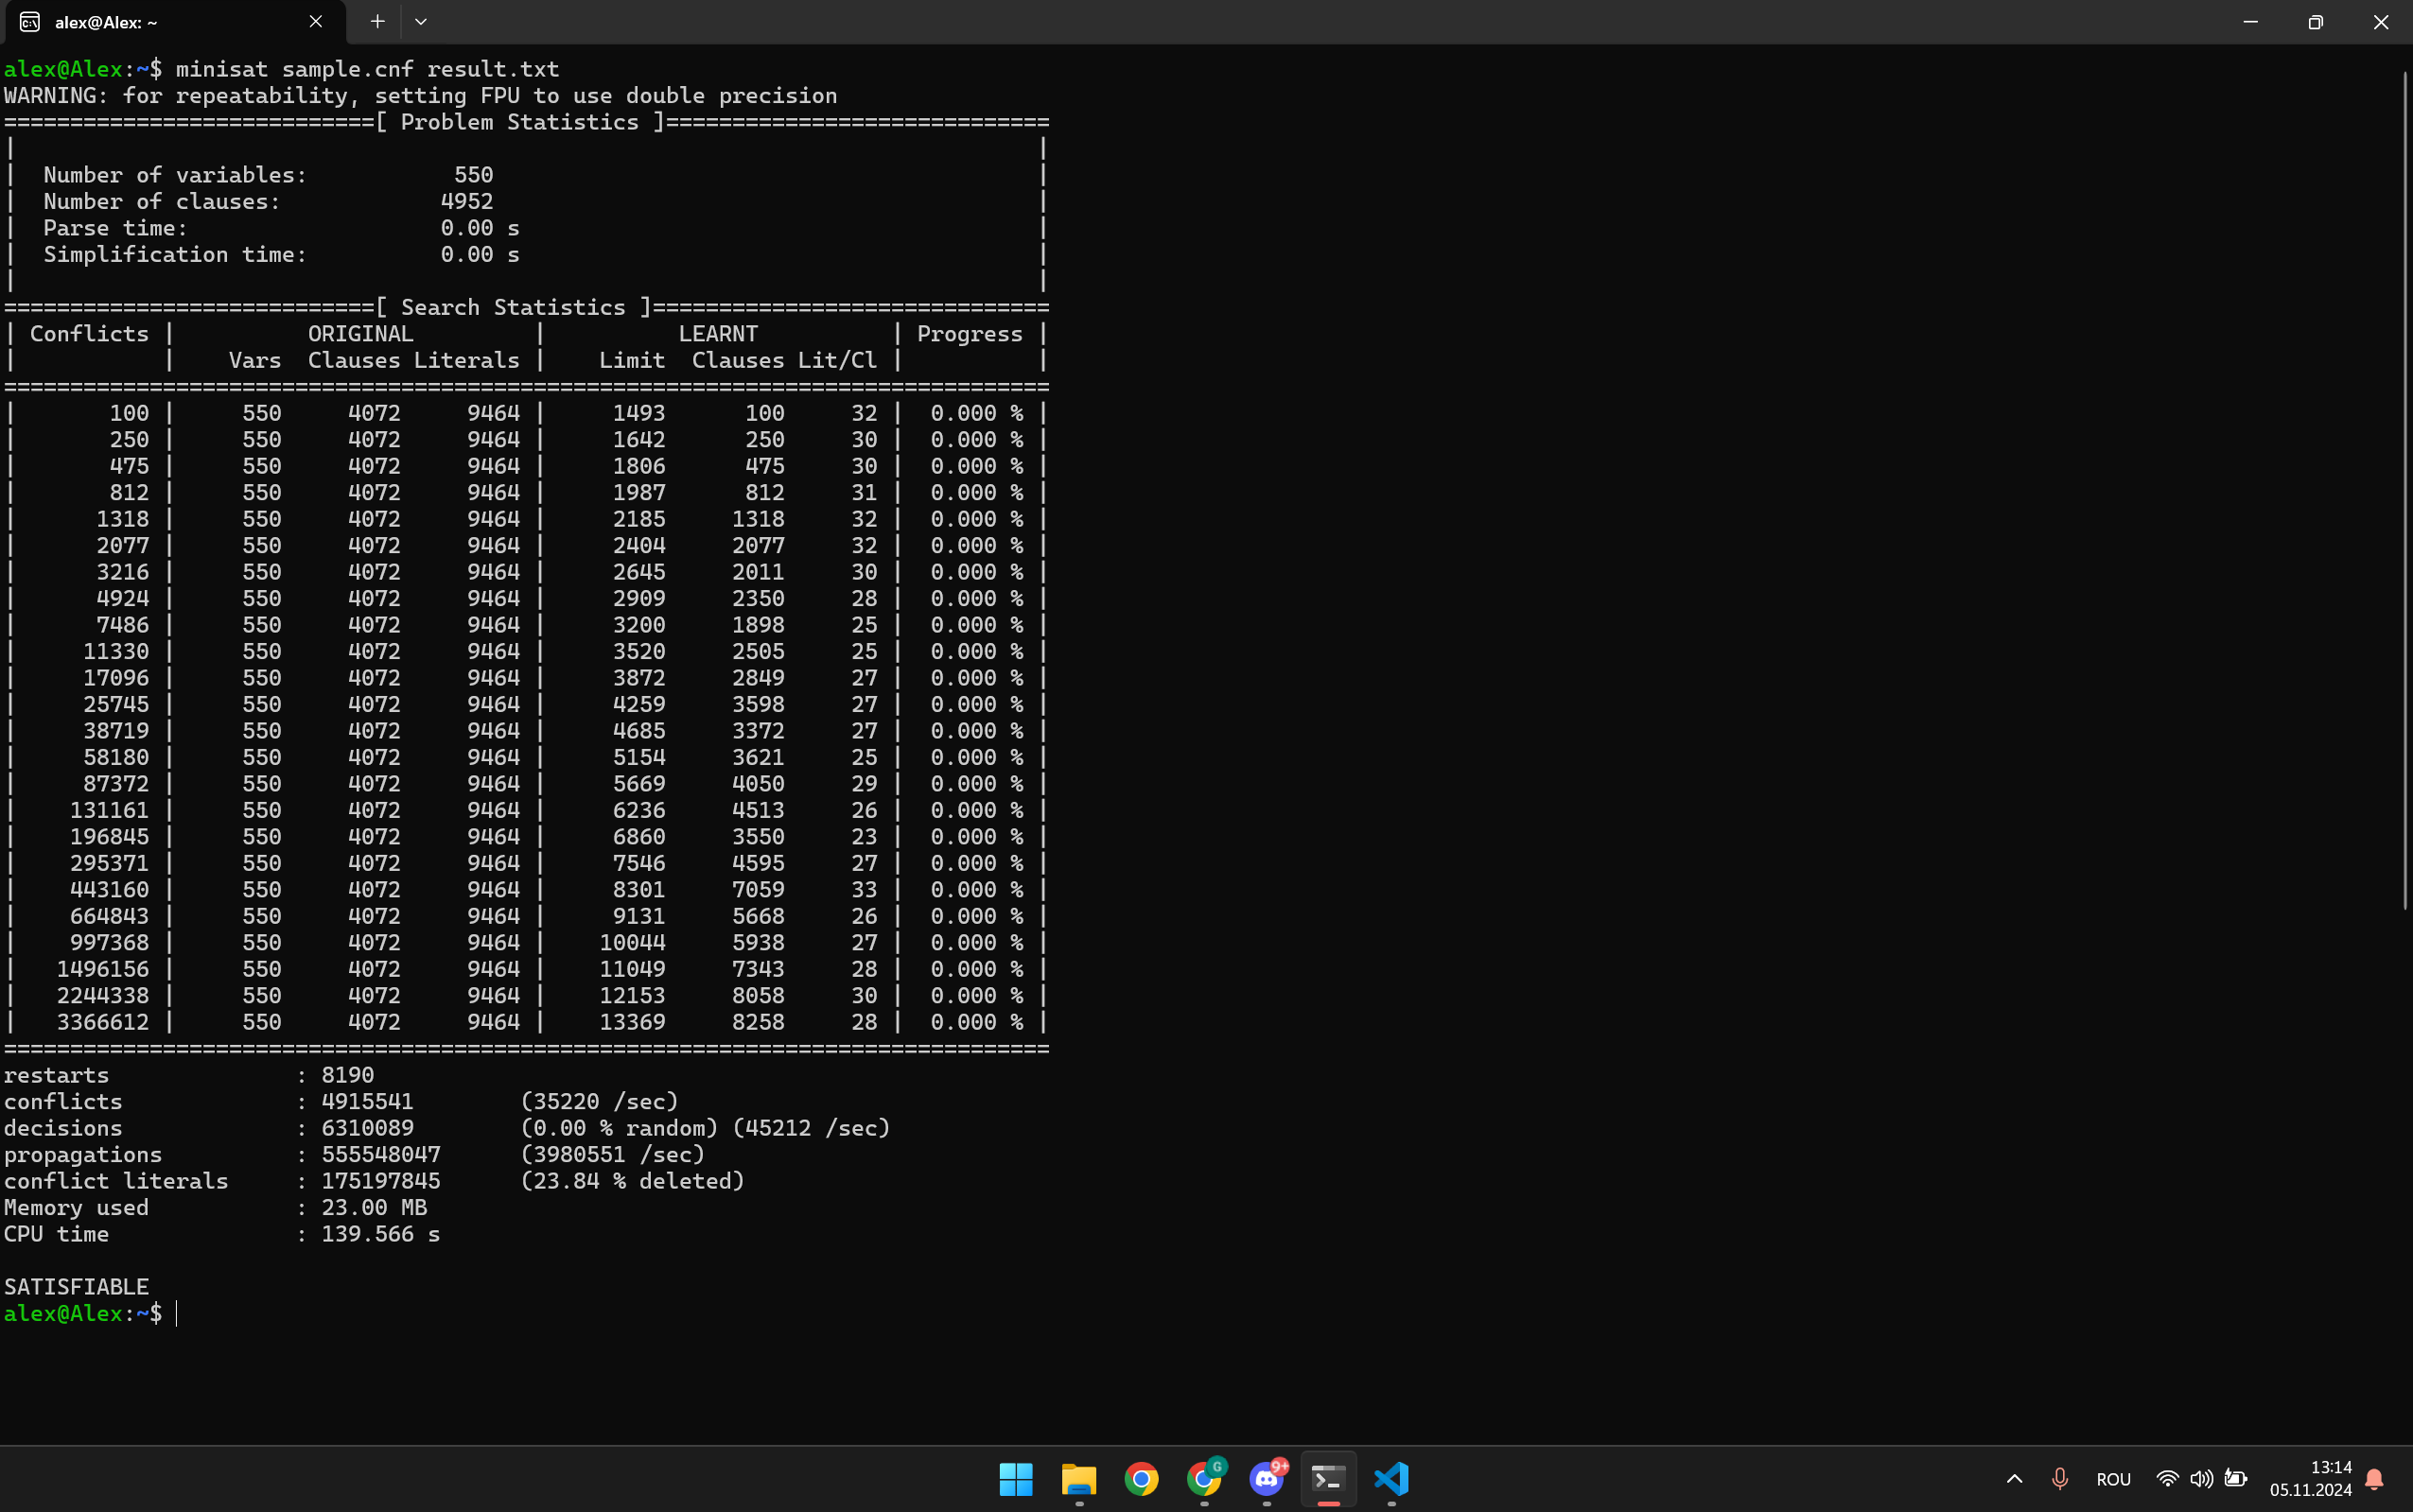
\includegraphics[width=12cm, height=5.7cm]{fig2.png}
\caption{MiniSat benchmark.} 
\label{fig2}
\end{figure}
\newpage

\begin{credits}
\subsubsection{\ackname} 

\subsubsection{\discintname}

\end{credits}
%
% ---- Bibliography ----
%
% BibTeX users should specify bibliography style 'splncs04'.
% References will then be sorted and formatted in the correct style.
%
% \bibliographystyle{splncs04}
% \bibliography{mybibliography}
%
\newpage
{\noindent \huge \listoffigures \par}
{\noindent \huge \textbf{List of acronyms}\par}

\begin{acronym}
 \acro{SAT}{Boolean satisfiability problem}
 \acro{e.g.}{example}
 \acro{NP-complete}{Nondeterministic Polynomial-Time complete}
 \acro{EDA}{electronic design automation}
 \acro{DPLL}{Davis Putnam Logemann Loveland}
 \acro{CDCL}{conflict-driven clause learning}
 \acro{UML}{Unified Modeling Language}
 \acro{CNF}{Conjunctive Normal Form}
  \acro{WSL}{Windows Subsystem for Linux}
\end{acronym}
\begin{thebibliography}{8}
\bibitem{sat-solver}
Authors: Niklas Een, Niklas Sorensson; Institute: Chalmers University of Technology, Sweden; Paper title: An Extensible SAT-solver[extended version 1.2]

\bibitem{minisat}
MiniSat documentation, \url{http://minisat.se/Main.html}

\end{thebibliography}
\end{document}